\documentclass[a4paper,12pt]{report}
\usepackage[T1]{fontenc}
\usepackage[utf8]{inputenc}
\usepackage{pslatex}
\usepackage{lmodern}
\usepackage{helvet}
\usepackage{geometry}
\usepackage{graphicx}
\usepackage{sectsty}
\usepackage{fancyhdr}
\usepackage{titlesec}
\usepackage{fixltx2e}
\usepackage{acronym}
\usepackage[titles]{tocloft}
\usepackage{amsmath}
\usepackage{amssymb}
\usepackage{cases}
\usepackage{cite}
\usepackage[export]{adjustbox}
\usepackage{url}
\usepackage{rotating} 
\usepackage{setspace}
\usepackage{booktabs}
\chapterfont{\large\centering}
\sectionfont{\normalsize}
\subsectionfont{\normalsize}
\linespread{1.5}
\geometry{a4paper,left=3cm,right=2cm,top=2cm,bottom=2cm}
\setcounter{tocdepth}{2}
\usepackage{amsmath}

\begin{document}
\renewcommand\abstractname{ABSTRACT}
\begin{abstract}
\thispagestyle{empty}
\paragraph{}  
Chatbot are software agents that interact with the user in a conversation. The main goal of their creation was to resemble a human being in the way they perform said interaction, trying to make the user think he/she is writing to another human being. The modular chatbot is an easily adaptable chatbot system to suit specific purposes. The bot will read and understand the messages sent to it and formulate effective responses to converse with the user. The bot uses a Deep Neural Network to learn conversations in its domain. The incoming messages are analysed by the  Deep Neural Network and replies are formulated. The bot uses the open source TFLearn framework built on tensorflow for python to implement the neural network. The chatbot will be modular in the sense that by using different domain specific data sets to train the neural network the bot can be adapted for different domains. The engine being completely separate from preprocessing multiple interfaces can be plugged on top of the chatbot core.
\end{abstract}

\pagenumbering{roman}
\setcounter{page}{1}
\setcounter{tocdepth}{1}
\renewcommand\contentsname{CONTENTS}
\tableofcontents
\newpage
\vspace*{2.52cm} \hspace*{-0.88cm}
\addcontentsline{toc}{chapter}{LIST OF ABBREVIATIONS}
\hspace*{4.3cm}
\textbf{{\large LIST OF ABBREVIATIONS}}\\
\vspace*{0.5cm}
\begin{acronym}[AWGN]
	\acro{DNN}{Deep Neural Network}
	\acro{API}{Application Programming Interface}
	\acro{APK}{Application Program Kit}
	\acro{ART}{Android Runtime}	
	\acro{BLE}{Bluetooth Low Energy}
	\acro{GPS}{Global Positioning System}
	\acro{JDK}{Java Development Kit}
	\acro{JIT}{Just in Time}
	\acro{NFC}{Near Field Communication}  
	\acro{PoI}{Point of Interest}
	\acro{RSSI}{Received Signal Strength Indicator}
	\acro{SDK}{Software Development Kit}
	\acro{SoC}{System on Chip}
	\acro{UUID}{Universal Unique Identifier}
\end{acronym}
\newpage
\addcontentsline{toc}{chapter}{LIST OF FIGURES}
\renewcommand\listfigurename{LIST OF FIGURES}
\listoffigures
\newpage
\addcontentsline{toc}{chapter}{LIST OF TABLES}
\renewcommand\listtablename{LIST OF TABLES}
\listoftables
\newpage
\pagenumbering{arabic}
\setcounter{page}{1}
\renewcommand\chaptername{CHAPTER}
\chapter{INTRODUCTION}
\paragraph{}Wireless Multi-level Indoor Positioning System is a system to locate objects or people inside a building using radio waves, magnetic fields, acoustic signals, or other sensory information collected by mobile devices. With increasing popularity over recent years, indoor location positioning systems provide a new layer of automation called automatic object location detection. These systems have varied applications like community settlement planning, military applications, surveillance, monitoring, mining, travelling and development of location-based services. Nowadays, when satellite navigation systems such as GPS, GLONASS, or Galileo are available for everyone, it is usually not a problem to locate a person or a mobile device outside. A situation can get more complicated in high-density urban areas with rare line-of-sight to the satellites of the corresponding system. The situation is most complicated inside buildings with no line-of-sight. In such cases, other solutions are employed, usually those based on radio networks (e.g., IEEE 802.11-WiFi) and packets of signal strengths of individual WiFi devices which transmit their signals inside a building. Another factor which can be adjusted quite easily is the number of radio transmitters and their positions. A typical situation is that there already are some WiFi access points in the building which more or less cover the building with the radio signal which can be used for localization. To increase the accuracy of the localization, it is possible to install more transmitters which would enrich the individual signal packet or cover the places which are poorly covered by the existing WiFi network. Our project deal with the Bluetooth Low Energy (BLE) technology which can be a very good alternative supplementing WiFi access points. Their combination will allow more accurate localization. The key advantage of BLE comprises low energy consumption which allows the transmitters—called beacons—to be powered continuously from batteries from months to years. This also makes it possible to place the beacons in the spots where WiFi access points would be difficult to power.
\section{Beacon Technology}
\paragraph{}iBeacon is Apple’s brand name of the technology based on the microlocalization and the interaction of a mobile device in the physical world. This technology can be considered to be the next development stage of the QR code technology or, alternatively, the NFC technology. beacon uses the Bluetooth Low Energy standard which is a part of a new version of Bluetooth 4.0. Sometimes, the terms Bluetooth Smart, Bluetooth LE, BTLE, and just BLE are used. It is a technology developed by Nokia (originally, the technology was named Wibree; in 2010 BLE was standardized) and in contrast to the previous versions of Bluetooth, dramatically lower consumption is typical for BLE. Also the way how the (peripheral) device announces its existence to the other devices is the opposite from how it is in the original Bluetooth Classic. BLE enables a peripheral device to transmit an advertisement packet without being paged by the master (central) device. Thanks to this communication model, it is possible to construct energy-efficient transmitters—BLE beacons or beacons according to Apple.

\paragraph{}iBeacon is a small device which transmits particular information in a defined radius and in regular intervals. As soon as a mobile device (a smartphone) gets within this radius, it can receive such information and, based on this, it can perform an action. Considering low consumption of BLE, such a device can be powered by a coin battery for up to two years. Of course, the battery life depends on the transmitter output power (TX power) and advertising interval settings.

\paragraph{}The Beacon technology is going to be adopted by shop marketers. A visitor with a BLE-enabled smartphone may be notified of special offers, discounts, information, and so forth based on his/her position or proximity to a beacon. It finds similar use in museums and exhibition halls.
\newpage
\section{Android Support for BLE}
\paragraph{}Android platform was chosen for testing the whole solution because it is the most widely used operating system for smartphones. Android offers BLE support from version 4.3 (API level 18). From version 5.0 (API level 21) the BLE-related API had been revised and extracted to a separate android.bluetooth.le package. The applications have to be granted both BLUETOOTH and BLUETOOTH\_ADMIN system permissions to use BLE API. API level 18 supports communication with BLE peripheral devices only—that is, scanning devices, enumerating device’s services, and sending or receiving the data to or from such devices. API level 21 further opens the possibility for a smartphone or a tablet (depending on hardware support) to act as a Bluetooth Low Energy peripheral device, that is, to advertise itself as a BLE device and to offer services to other devices.
\paragraph{}The most important function for BLE indoor localization is scanning of the available BLE devices in the neighborhood. For this purpose, API level 18 offers startLeScan() and stopLeScan() methods of the BluetoothManager class. The scanning process is asynchronous and every device found is reported to an instance of the LeScanCallback callback class. The scanned device is represented by the BluetoothDevice class which includes its MAC address, byte-array scan record (containing UUID, etc.), and RSSI. API level 21 moves the process of low energy scanning into the separate BluetoothLeScanner class. Its instance is obtained by calling the getBluetoothLeScanner() method of the BluetoothAdapter class. In contrast to API level 18, it is possible to specify even more detailed parameters of scanning. Unfortunately, implementation of the above mentioned classes and underlying system libraries can vary across different vendors. The most common issue is that BLE devices are not reported repeatedly during the scanning process which is a condition necessary for localization. For this reason it is necessary to implement a mechanism which starts and stops scanning repeatedly in a given time interval. It is also possible to use available libraries, for example, Android Beacon Library (https://github.com/AltBeacon/android-beacon-library/), which provides CycledLeScanner class that encapsulates this mechanism.
\newpage
\section{Problem Statement}
\paragraph{}The existing positioning system solutions are GPS and WiFi technology. While trying to focus those on the indoor postioning system, these technologies have some drawbacks.
\paragraph{}Global positioning system (GPS), or its differential complement DGPS, is one of the most successful positioning systems in outdoor environments. However, poor coverage of satellite signal for indoor environments decreases its accuracy and makes it unsuitable for indoor location estimation. GPS technology can’t be used to know the exact position of the user. Using GPS, it is not possible for the system to determine the exact floor in which the user is residing. GPS, being the most popular technology in location determination, is not suitable for indoor location estimation as users’ devices might not have GPS interface, and even if they do, the devices are unable to catch radio waves from satellites if the user is indoor of some building. Moreover, GPS requires a strong computing platform which is not available in sensor networks. Sensor nodes, being lowcomputing power units, can efficiently perform only basic arithmetic operations. The execution of complex arithmetic operation may quickly deplete the battery of the sensor node which is practically an undesirable feature.
\paragraph{}With the advancement of wireless and embedded technology, local wireless networks are commonplace, and in times when these technologies have fostered the smartphone markets to flourish, integration of wireless systems with embedded devices like smartphones have been widespread and have opened new areas for powerful computations and communication capabilities using built-in sensors for various functions. Wi-Fi signals need more access points to be deployed and more number of signal samples has to be used. But this requires more energy consumption. WiFi technology can create a mesh. But if any router fails, the whole system will fail. And also, it can’t communicate with one another.
\paragraph{}Bluetooth-based indoor localization is not a novel idea. Due to the limitation of the original Bluetooth specification (now called Bluetooth Classic), this approach has not been widely used. The time required for obtaining a sufficient number of nearby Bluetooth devices was not satisfactory due to the lengthy process of discovery. Likewise, energy and economic demands of Bluetooth infrastructure were high compared to WiFi-based infrastructure, which also served other purposes.
\section{Objective}
\paragraph{}With the advent of Bluetooth 4.0 (including BLE/Bluetooth Smart) in 2010, the indoor positioning system have emerged. Due to low energy consumption and configuration options (regarding the advertising interval and the transmitter output power), the utilisation of this technology is much more promising, not only in comparison with previous versions of Bluetooth, but also in comparison with today’s widespread WiFi-positioning. BLE is more accurate at identical places than WiFi.
\paragraph{}The main objective of this system is to navigate the user to the desired destination via BLE devices known as Beacons. Beacons advertise their MAC address, UUID, Major, Minor and RSSI values periodically. From the RSSI value, we can determine the exact position of the user. 
\section{Utilizing BLE in Indoor Positioning System}
\paragraph{}WiFi networks are commonly being used for localization inside buildings. A building is usually a complicated system regarding WiFi signal propagation due to the materials used. That is why areas with no WiFi signal may appear in the buildings despite high concentration of efficient WiFi access points. In such areas it is not possible to collect signal packets because they would contain no signals measured from the surrounding WiFi networks. These areas can additionally be covered by other transmitters. For this purpose, BLE beacons can be used. They transmit a Bluetooth signal instead of a WiFi signal. While powered by batteries, they can be placed in less accessible places where there are no power sockets or other forms of supply, such as ethernet cables, allowing to use power-over-ethernet. When placing the beacons it is necessary to care about the radiation pattern of a given device and also about possible attenuation elements in the environment.

\paragraph{}Due to the low price of beacons, their small size, and independence of an external power supply (no additional cables required), they seem to be suitable supplements to an existing WiFi network in a building. Areas covered with weak WiFi signal or with a small number of WiFi transmitters contained in one fingerprint can thus be enriched by new BLE transmitters. Then, the fingerprint can also contain the measured RSSIs of these BLE devices in addition to the RSSIs of WiFi signals.

\paragraph{}Beacons have another advantage: thanks to support by mobile operating systems, they can be used for energy-efficient geofencing enabling a mobile application to be activated based on approaching an iBeacon by a smartphone. The whole process at the iOS platform does not require the application to be active and thanks to this it is possible to optimize it so the energy consumption of the mobile device is minimized and the endurance of the battery is maximized. Estimote has also established a new term in this field—nearables—for their BLE beacons equipped with additional sensors.

\vspace{2cm}
\begin{figure}[!h]
	\begin{center}
		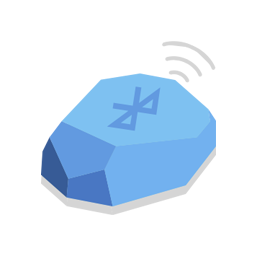
\includegraphics[width=.5\textwidth]{beacon.png}    
		\caption{Beacon}
		\label{fig13}
	\end{center}
\end{figure}

\renewcommand\chaptername{CHAPTER}
\chapter{REQUIREMENT ANALYSIS}
\paragraph{} Mainly, we have two types of requirements. They are hardware and software requirements.
\begin{itemize}
	\item Hardware Requirements
	\begin{itemize}
		\item Beacons
		\item Android Phone
	\end{itemize}
	\item Software Requirements
	\begin{itemize}
		\item Android Studio
	\end{itemize}
\end{itemize}
\section{Android Operating System}
\paragraph{} Android is a mobile operating system developed by Google, based on the Linux kernel and designed primarily for touchscreen mobile devices such as smartphones and tablets. Android's user interface is mainly based on direct manipulation, using touch gestures that loosely correspond to real-world actions, such as swiping, tapping and pinching, to manipulate on-screen objects, along with a virtual keyboard for text input. In addition to touchscreen devices, Google has further developed Android TV for televisions, Android Auto for cars, and Android Wear for wrist watches, each with a specialized user interface. Variants of Android are also used on notebooks, game consoles, digital cameras, and other electronics.
\paragraph{} Initially developed by Android Inc., which Google bought in 2005, Android was unveiled in 2007, along with the founding of the Open Handset Alliance – a consortium of hardware, software, and telecommunication companies devoted to advancing open standards for mobile devices. Beginning with the first commercial Android device in September 2008, the operating system has gone through multiple major releases, with the current version being 7.0 ``Nougat'', released in August 2016. Android applications (``apps'') can be downloaded from the Google Play store, which features over 2.7 million apps as of February 2017. Android has been the best-selling OS on tablets since 2013, and runs on the vast majority of smartphones. In September 2015, Android had 1.4 billion monthly active users, and it has the largest installed base of any operating system.
\paragraph{} Android's source code is released by Google under an open source license, although most Android devices ultimately ship with a combination of free and open source and proprietary software, including proprietary software required for accessing Google services. Android is popular with technology companies that require a ready-made, low-cost and customizable operating system for high-tech devices. Its open nature has encouraged a large community of developers and enthusiasts to use the open-source code as a foundation for community-driven projects, which deliver updates to older devices, add new features for advanced users or bring Android to devices originally shipped with other operating systems. The extensive variation of hardware in Android devices causes significant delays for software upgrades, with new versions of the operating system and security patches typically taking months before reaching consumers, or sometimes not at all. The success of Android has made it a target for patent and copyright litigation as part of the so-called ``smartphone wars'' between technology companies.
\subsection{Interface}
\paragraph{}Android's default user interface is mainly based on direct manipulation, using touch inputs that loosely correspond to real-world actions, like swiping, tapping, pinching, and reverse pinching to manipulate on-screen objects, along with a virtual keyboard. Game controllers and full-size physical keyboards are supported via Bluetooth or USB. The response to user input is designed to be immediate and provides a fluid touch interface, often using the vibration capabilities of the device to provide haptic feedback to the user. Internal hardware, such as accelerometers, gyroscopes and proximity sensors are used by some applications to respond to additional user actions, for example adjusting the screen from portrait to landscape depending on how the device is oriented, or allowing the user to steer a vehicle in a racing game by rotating the device, simulating control of a steering wheel.
\paragraph{}Android devices boot to the homescreen, the primary navigation and information ``hub'' on Android devices, analogous to the desktop found on personal computers. Android homescreens are typically made up of app icons and widgets; app icons launch the associated app, whereas widgets display live, auto-updating content, such as a weather forecast, the user's email inbox, or a news ticker directly on the homescreen. A homescreen may be made up of several pages, between which the user can swipe back and forth. Third-party apps available on Google Play and other app stores can extensively re-theme the homescreen, and even mimic the look of other operating systems, such as Windows Phone. Most manufacturers customize the look and features of their Android devices to differentiate themselves from their competitors.
\paragraph{}Along the top of the screen is a status bar, showing information about the device and its connectivity. This status bar can be ``pulled'' down to reveal a notification screen where apps display important information or updates. Notifications are ``short, timely, and relevant information about your app when it’s not in use'', and when tapped, users are directed to a screen inside the app relating to the notification. Beginning with Android 4.1 ``Jelly Bean'', ``expandable notifications'' allow the user to tap an icon on the notification in order for it to expand and display more information and possible app actions right from the notification. All Apps screen lists all installed applications, with the ability for users to drag an app from the list onto the home screen. A Recent screen lets users switch between recently used apps.
\subsection{Applications}
\paragraph{}Applications (``apps''), which extend the functionality of devices, are written using the Android software development kit (SDK) and, often, the Java programming language. Java may be combined with C/C++, together with a choice of non-default runtimes that allow better C++ support. The Go programming language is also supported, although with a limited set of application programming interfaces (API).
\paragraph{}The SDK includes a comprehensive set of development tools, including a debugger, software libraries, a handset emulator based on QEMU, documentation, sample code, and tutorials. Initially, Google's supported integrated development environment (IDE) was Eclipse using the Android Development Tools (ADT) plugin; in December 2014, Google released Android Studio, based on IntelliJ IDEA, as its primary IDE for Android application development. Other development tools are available, including a native development kit (NDK) for applications or extensions in C or C++, Google App Inventor, a visual environment for novice programmers, and various cross platform mobile web applications frameworks. In January 2014, Google unveiled an framework based on Apache Cordova for porting Chrome HTML 5 web applications to Android, wrapped in a native application shell.
\paragraph{}Android has a growing selection of third-party applications, which can be acquired by users by downloading and installing the application's APK (Android application package) file, or by downloading them using an application store program that allows users to install, update, and remove applications from their devices. Google Play Store is the primary application store installed on Android devices that comply with Google's compatibility requirements and license the Google Mobile Services software. Google Play Store allows users to browse, download and update applications published by Google and third-party developers; as of July 2013, there are more than one million applications available for Android in Play Store. As of July 2013, 50 billion applications have been installed. Some carriers offer direct carrier billing for Google Play application purchases, where the cost of the application is added to the user's monthly bill.
\paragraph{}Due to the open nature of Android, a number of third-party application marketplaces also exist for Android, either to provide a substitute for devices that are not allowed to ship with Google Play Store, provide applications that cannot be offered on Google Play Store due to policy violations, or for other reasons. Examples of these third-party stores have included the Amazon Appstore, GetJar, and SlideMe. F-Droid, another alternative marketplace, seeks to only provide applications that are distributed under free and open source licenses.
\subsection{Memory Management}
\paragraph{}Since Android devices are usually battery-powered, Android is designed to manage processes to keep power consumption at a minimum. When an application is not in use the system suspends its operation so that, while available for immediate use rather than closed, it does not use battery power or CPU resources. Android manages the applications stored in memory automatically: when memory is low, the system will begin invisibly and automatically closing inactive processes, starting with those that have been inactive for longest. Lifehacker reported in 2011 that third-party task killers were doing more harm than good.
\subsection{Virtual Reality}
\paragraph{}At Google I/O on May 2016, Google announced Daydream, a virtual reality platform that relies on a smartphone and provides VR capabilities through a virtual reality headset and controller designed by Google itself. The platform is built into Android starting with Android Nougat, differentiating from standalone support for VR capabilities. The software is available for developers, and was released in 2016.
\subsection{Hardware}
\paragraph{}The main hardware platform for Android is the ARM (ARMv7 and ARMv8-A architectures), with x86, MIPS and MIPS64, and x86-64 architectures also officially supported in later versions of Android. The unofficial Android-x86 project provided support for the x86 architectures ahead of the official support. MIPS architecture was also supported before Google did. Since 2012, Android devices with Intel processors began to appear, including phones and tablets. While gaining support for 64-bit platforms, Android was first made to run on 64-bit x86 and then on ARM64. Since Android 5.0 "Lollipop", 64-bit variants of all platforms are supported in addition to the 32-bit variants.
\paragraph{}Requirements for the minimum amount of RAM for devices running Android 5.1 range from 512 MB of RAM for normal-density screens, to about 1.8 GB for high-density screens. The recommendation for Android 4.4 is to have at least 512 MB of RAM, while for "low RAM" devices 340 MB is the required minimum amount that does not include memory dedicated to various hardware components such as the baseband processor. Android 4.4 requires a 32-bit ARMv7, MIPS or x86 architecture processor (latter two through unofficial ports), together with an OpenGL ES 2.0 compatible graphics processing unit (GPU). Android supports OpenGL ES 1.1, 2.0, 3.0, 3.1 and as of latest major version, 3.2 and Vulkan. Some applications may explicitly require a certain version of the OpenGL ES, and suitable GPU hardware is required to run such applications.
\paragraph{}Android devices incorporate many optional hardware components, including still or video cameras, GPS, orientation sensors, dedicated gaming controls, accelerometers, gyroscopes, barometers, magnetometers, proximity sensors, pressure sensors, thermometers, and touchscreens. Some hardware components are not required, but became standard in certain classes of devices, such as smartphones, and additional requirements apply if they are present. Some other hardware was initially required, but those requirements have been relaxed or eliminated altogether. For example, as Android was developed initially as a phone OS, hardware such as microphones were required, while over time the phone function became optional. Android used to require an autofocus camera, which was relaxed to a fixed-focus camera if present at all, since the camera was dropped as a requirement entirely when Android started to be used on set-top boxes.
\paragraph{}In addition to running on smartphones and tablets, several vendors run Android natively on regular PC hardware with a keyboard and mouse. In addition to their availability on commercially available hardware, similar PC hardware-friendly versions of Android are freely available from the Android-x86 project, including customized Android 4.4. Using the Android emulator that is part of the Android SDK, or third-party emulators, Android can also run non-natively on x86 architectures. Chinese companies are building a PC and mobile operating system, based on Android, to "compete directly with Microsoft Windows and Google Android". The Chinese Academy of Engineering noted that "more than a dozen" companies were customising Android following a Chinese ban on the use of Windows 8 on government PCs.
\subsection{Development}
\paragraph{}Android is developed by Google until the latest changes and updates are ready to be released, at which point the source code is made available to the Android Open Source Project. This source code can be found without modification on select devices, mainly the Nexus series of devices. The source code is, in turn, adapted by original equipment manufacturers (OEMs) to run on their hardware. Android's source code does not contain the often proprietary device drivers that are needed for certain hardware components. 
\paragraph{}In 2007, the green Android logo was designed for Google by graphic designer Irina Blok. The design team was tasked with a project to create a universally identifiable icon with the specific inclusion of a robot in the final design. After numerous design developments based on science fiction and space movies, the team eventually sought inspiration from the human symbol on restroom doors and modified the figure into a robot shape. As Android is open-source, it was agreed that the logo should be likewise, and since its launch the green logo has been reinterpreted into countless variations on the original design.
\subsection{Linux Kernal}
\paragraph{}Android's kernel is based on one of the Linux kernel's long-term support (LTS) branches. Since April 2014, Android devices mainly use versions 3.4, 3.10 or 3.18 of the Linux kernel. The specific kernel version depends on the actual Android device and its hardware platform; Android has used various kernel versions since the version 2.6.25 that was used in Android 1.0.
\paragraph{}Android's variant of the Linux kernel has further architectural changes that are implemented by Google outside the typical Linux kernel development cycle, such as the inclusion of components like Binder, ashmem, pmem, logger, wakelocks, and different out-of-memory (OOM) handling. Certain features that Google contributed back to the Linux kernel, notably a power management feature called ``wakelocks'', were rejected by mainline kernel developers partly because they felt that Google did not show any intent to maintain its own code. Google announced in April 2010 that they would hire two employees to work with the Linux kernel community, but Greg Kroah-Hartman, the current Linux kernel maintainer for the stable branch, said in December 2010 that he was concerned that Google was no longer trying to get their code changes included in mainstream Linux. Some Google Android developers hinted that ``the Android team was getting fed up with the process,'' because they were a small team and had more urgent work to do on Android.
\paragraph{}In August 2011, Linus Torvalds said that ``eventually Android and Linux would come back to a common kernel, but it will probably not be for four to five years''. In December 2011, Greg Kroah-Hartman announced the start of Android Mainlining Project, which aims to put some Android drivers, patches and features back into the Linux kernel, starting in Linux 3.3. Linux included the autosleep and wakelocks capabilities in the 3.5 kernel, after many previous attempts at merger. The interfaces are the same but the upstream Linux implementation allows for two different suspend modes: to memory (the traditional suspend that Android uses), and to disk (hibernate, as it is known on the desktop). Google maintains a public code repository that contains their experimental work to re-base Android off the latest stable Linux versions.
\paragraph{}The flash storage on Android devices is split into several partitions, such as /system for the operating system itself, and /data for user data and application installations. In contrast to desktop Linux distributions, Android device owners are not given root access to the operating system and sensitive partitions such as /system are read-only. However, root access can be obtained by exploiting security flaws in Android, which is used frequently by the open-source community to enhance the capabilities of their devices, but also by malicious parties to install viruses and malware.
\paragraph{}Android is a Linux distribution according to the Linux Foundation, Google's open-source chief Chris DiBona, and several journalists. Others, such as Google engineer Patrick Brady, say that Android is not Linux in the traditional Unix-like Linux distribution sense; Android does not include the GNU C Library (it uses Bionic as an alternative C library) and some of other components typically found in Linux distributions. 
\subsection{Software Stack}
\paragraph{}On top of the Linux kernel, there are the middleware, libraries and APIs written in C, and application software running on an application framework which includes Java-compatible libraries. Development of the Linux kernel continues independently of other Android's source code bases.
\paragraph{}Until version 5.0, Android used Dalvik as a process virtual machine with trace-based just-in-time (JIT) compilation to run Dalvik ``dex-code'' (Dalvik Executable), which is usually translated from the Java bytecode. Following the trace-based JIT principle, in addition to interpreting the majority of application code, Dalvik performs the compilation and native execution of select frequently executed code segments (``traces'') each time an application is launched. Android 4.4 introduced Android Runtime (ART) as a new runtime environment, which uses ahead-of-time (AOT) compilation to entirely compile the application bytecode into machine code upon the installation of an application. In Android 4.4, ART was an experimental feature and not enabled by default; it became the only runtime option in the next major version of Android 5.0.
\begin{figure}[!h]
	\begin{center}
		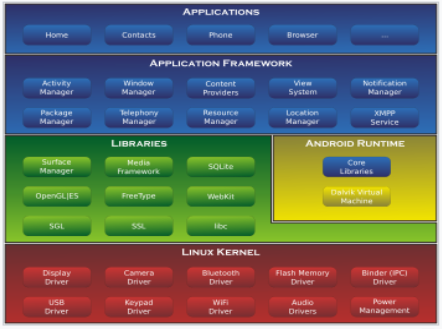
\includegraphics[width=.75\textwidth]{arc.png}    
		\caption{Android's Architecture Diagram}
		\label{fig1}
	\end{center}
\end{figure}
\paragraph{}For its Java library, the Android platform uses a subset of the now discontinued Apache Harmony project. In December 2015, Google announced that the next version of Android would switch to a Java implementation based on OpenJDK.
\paragraph{}Android's standard C library, Bionic, was developed by Google specifically for Android, as a derivation of the BSD's standard C library code. Bionic itself has been designed with several major features specific to the Linux kernel. The main benefits of using Bionic instead of the GNU C Library (glibc) or uClibc are its smaller runtime footprint, and optimization for low-frequency CPUs. At the same time, Bionic is licensed under the terms of the BSD licence, which Google finds more suitable for the Android's overall licensing model.
\paragraph{}Aiming for a different licensing model, toward the end of 2012, Google switched the Bluetooth stack in Android from the GPL-licensed BlueZ to the Apache-licensed BlueDroid. Android does not have a native X Window System by default, nor does it support the full set of standard GNU libraries. This made it difficult to port existing Linux applications or libraries to Android, until version r5 of the Android Native Development Kit brought support for applications written completely in C or C++. Libraries written in C may also be used in applications by injection of a small shim and usage of the JNI. Since Marshmallow, ``Toybox'', a collection of command line utilities (mostly for use by apps, as Android doesn't provide a command line interface by default), replaced similar ``Toolbox'' collection.
\paragraph{}Android has another operating system, Trusty OS, within it, as a part of ``Trusty'' ``software components supporting a Trusted Execution Environment (TEE) on mobile devices''. ``Trusty and the Trusty API are subject to change. Applications for the Trusty OS can be written in C/C++ (C++ support is limited), and they have access to a small C library. All Trusty applications are single-threaded; multithreading in Trusty userspace currently is unsupported''. Third-party application development is not supported in the current version, and software running on the OS and processor for it, run the ``DRM framework for protected content.  There are many other uses for a TEE such as mobile payments, secure banking, full-disk encryption, multi-factor authentication, device reset protection, replay-protected persistent storage, wireless display (``cast'') of protected content, secure PIN and fingerprint processing, and even malware detection.'' 
\section{Android Studio}
\paragraph{}Android Studio is the official integrated development environment (IDE) for the Android platform. It was announced on May 16, 2013 at the Google I/O conference.
\paragraph{}Android Studio was in early access preview stage starting from version 0.1 in May 2013, then entered beta stage starting from version 0.8 which was released in June 2014. The first stable build was released in December 2014, starting from version 1.0. 
\paragraph{}Based on JetBrains' IntelliJ IDEA software, Android Studio is designed specifically for Android development. It is available for download on Windows, macOS and Linux, and replaced Eclipse Android Development Tools (ADT) as Google's primary IDE for native Android application development.
\begin{figure}[!h]
	\begin{center}
		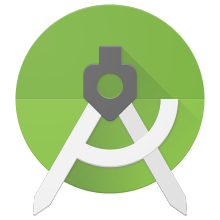
\includegraphics[width=.5\textwidth]{as.png}    
		\caption{Android Studio}
		\label{fig2}
	\end{center}
\end{figure}
\subsection{Features}
\paragraph{}New features are expected to be rolled out with each release of Android Studio. The following features are provided in the current stable version :
\begin{itemize}
	\item Gradle-based build support
	\item Android-specific refactoring and quick fixes
	\item Lint tools to catch performance, usability, version compatibility and other problems
	\item ProGuard integration and app-signing capabilities
	\item Template-based wizards to create common Android designs and components
	\item A rich layout editor that allows users to drag-and-drop UI components, option to preview layouts on multiple screen configurations
	\item Support for building Android Wear apps
	\item Built-in support for Google Cloud Platform, enabling integration with Firebase Cloud Messaging (Earlier `Google Cloud Messaging') and Google App Engine
	\item Android Virtual Device (Emulator) to run and debug apps
\end{itemize}
\subsection{System Requirements}
\paragraph{}The system requirements for installing Android Studio 2.x is given below :
\begin{table}[!h]
	\centering
	\caption{System Requirements for Android Studio 2.x}
	\label{table1}
	\begin{tabular}{|c|c|}
		\hline
		\textbf{Criterion} & \textbf{Description} \\
		\hline
		OS version & \begin{tabular}[c]{@{}l@{}}Windows 7 or later \\ Mac OS X 10.9.5 or later\\ GNOME or KDE Desktop\end{tabular}\\
		\hline
		RAM & 3 GB RAM minimum, 8 GB RAM Recommended\\
		\hline
		Disk Space & 500 MB disk space for Android Studio, atleast 1.5 GB for Android SDK\\
		\hline
		Java Version & JDK 8\\
		\hline
		Screen Resolution & 1280x800 minimum screen resolution\\
		\hline
	\end{tabular}
\end{table}
\newpage
\paragraph{} The system requirements for installing Android Studio 1.x is given below :
\begin{table}[!h]
	\centering
	\caption{System Requirements for Android Studio 1.x}
	\label{table2}
	\begin{tabular}{|c|c|}
		\hline
		\textbf{Criterion} & \textbf{Description} \\
		\hline
		OS version & \begin{tabular}[c]{@{}l@{}}Windows XP or later \\ Mac OS X 10.8.5 or later\\ GNOME or KDE Desktop\end{tabular}\\
		\hline
		RAM & 3 GB RAM minimum, 4 GB RAM Recommended\\
		\hline
		Disk Space & 500 MB disk space for Android Studio, atleast 1 GB for Android SDK\\
		\hline
		Java Version & JDK 7 or higher\\
		\hline
		Screen Resolution & 1280x800 minimum screen resolution\\
		\hline
	\end{tabular}
\end{table}
\renewcommand\chaptername{CHAPTER}
\chapter{DESIGN}
\section{Algorithm}
\paragraph{} We are developing an Android Application for Wireless Multi-level Indoor Positioning System in our college, which is based on BLE based technology Beacon pre-installed in the campus. Given in this section is the method of system implementation on Android environment in the form of a sample algorithm\\
\begin{enumerate}
	\item START
	\item Read user's desired destination and find source of the user.
	\item Repeat steps 3 to 5 while navigating 
	\item CHECK IF the beacon is not available in the fixed path, THEN \\indicate the user that he/she is in wrong direction.
	\item ELSE CHECK IF the user has reached destination THEN indicate the user that he/she has reached destination and exit the module.
	\item ELSE goto step 3.
	\item STOP
\end{enumerate}
\newpage
\section{Block Diagram}
\begin{figure}[!h]
	\begin{center}
		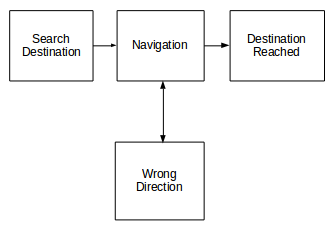
\includegraphics[width=.75\textwidth]{BD.png}    
		\caption{Block Diagram}
		\label{fig3}
	\end{center}
\end{figure}
\paragraph{} Fig. \ref{fig3} shows the block diagram of the system. The system consists of 4 modules.
\subsection{Search Destination Module}
\paragraph{}This module is done by the user for searching the desired destination. The user will select the desired destination through a dropdown list. The dropdown contains all the destinations. The user, after selecting the desired destination, will search for a path from source to destination. The source can be identified from his current position through RSSI value of the Beacons. The system searches BLE devices with a specific UUID. The BLE device with greater RSSI value is determined as the source as the user is nearer to that device. After identifying the source, the path from source to destination is shown. 
\subsection{Navigation Module}
\paragraph{}This module is for navigating the user to the desired destination from source through the path. If the user wants to turn left/right, the system will notify the user through text and audio output. The turns can be identified through the Beacons and the desired destination. Beacons advertises major, minor and RSSI values periodically. From the RSSI value, the system can determine whether the user is nearer or farther to the Beacon.
\newpage
\subsection{Wrong Direction Module}
\paragraph{}This module notifies the user that he/she is in wrong direction. While navigation, if the user is not in the desired direction, the system will notify the user through text and audio output. The identification of the wrong direction is through the major and minor values of the Beacons. If the next beacon is not found while searching BLE devices, it satisfies the condition that the user is in wrong direction.
\subsection{Destination Reached Module}
\paragraph{}This primarily notifies the user that he/she has reached the desired destination. The destination is identified using major, minor and RSSI values of the Beacon. When the destination has reached, the system will notify the user through text and audio output. The RSSI value is to determine the exact position of the user from the Beacon. If the user is nearer to the Beacon, then the RSSI value will be greater and vice versa.
\renewcommand\chaptername{CHAPTER}
\chapter{IMPLEMENTATION AND RESULTS}
\section{Using HM-10 BLE Modules as Low-Cost Beacons}
\paragraph{} The HM-10 is a readily available Bluetooth 4.0 module based on the Texas Instruments CC2540 or CC2541 Bluetooth Low Energy (BLE) System on Chip (SoC). The module design and firmware originated from the Jinan Huamao Technology Company (JNHuaMao), but is sold by various Chinese suppliers, and by several U.S. and European distributors. The modules shown here were purchased directly from ITead Studio’s iMall web site for only US\$6.50 each. They came pre-loaded with HM-10 Firmware version 526, but at the time I received them, version 528 (June 2014) was already available from the JNHuaMao download site, so I upgraded all the modules (more about how to do that later). As of September 2014 firmware version 531 was available.
\vspace{1cm}
\begin{figure}[!h]
	\begin{center}
		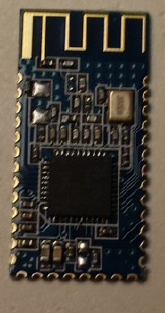
\includegraphics[width=.25\textwidth]{hm10.png}    
		\caption{HM-10 Module}.
		\label{fig4}
	\end{center}
\end{figure}
\paragraph{}The module is fairly small as seen in fig \ref{fig4} above. The contact spacing is 1.5 mm. Care should be taken when soldering wires to the module which will be necessary to connect it to a power source, and temporarily to a USB serial interface module and PC to configure the module as an iBeacon. The HM-10 is rated to operate at a supply voltage of 2.0 to 3.7 volts, and its I/O are 3.3V tolerant.
\section{Firmware Update}
\paragraph{}Before updating the HM-10 firmware, make sure have reliable connections to the module, and that the wires and cables cannot be accidentally knocked loose.
\begin{enumerate}
	\item  Using the Arduino serial monitor enter the command AT+SBLUP. The HM-10 should respond with OK+SBLUP. At this point the HM-10 is waiting for the firmware update. 
	\item Exit the serial monitor program. 
	\item Next, launch the firmware update program (the .exe file that you extracted from the zip file) most likely called HMSoft.exe. 
	\item In the COM Port field, enter the COM port number of the port connected to your HM-10. For example if it is COM3, enter 3 in the field. 
	\item Click on the “…” button for the Image File field, and select the .bin file name of the file that came in the zip file: HMSoft.bin. 
	\item Finally, click on Load Image button. 
	\item The firmware update will proceed and will take a couple of minutes. Do not interrupt the update process. Do not do anything else on the PC while the update is taking place to reduce the chances the process will be interrupted.
	\item When verification is complete, it may take a few seconds before the Download completed successfully message is displayed. 
\end{enumerate}
\newpage
\section{Beacon Configuration}
\paragraph{}The HM-10 uses an AT command set that requires very unusual timing when manually typing in commands from the PC. The commands are not terminated by a carriage return or line feed, and rely on a very short delay after the command line has been entered to complete.
\paragraph{}There have to type in a few commands to the HM-10 to configure it as an iBeacon. Use the Arduino serial monitor program to do this. In the following list, the bold initial text is the command that should type into the HM-10 and the rest is a comment on what it does. Each command will be acknowledged with an OK.
\begin{table}[!h]
	\centering
	\caption{AT Commands}
	\label{table3}
	\begin{tabular}{|c|c|}
		\hline
		\textbf{AT Commands} & \textbf{Description}\\
		\hline
		AT+RENEW & Restores factory defaults\\
		\hline
		AT+RESET & Reboot HM-10\\
		\hline
		AT & Wait for OK\\
		\hline
		AT+MARJ0x1234 &	Set iBeacon Major number to 0x1234 (hexadecimal)\\
		\hline
		AT+MINO0xFA01 &	Set iBeacon Minor number to 0xFA01 (hexadecimal)\\
		\hline
		AT+ADVI5 & Set advertising interval to 5 (546.25 milliseconds)\\
		\hline
		AT+NAMEDOPEY & Set HM-10 module name to DOPEY\\
		\hline
		AT+ADTY3 & Make non-connectable (save power)\\
		\hline
		AT+IBEA1 & Enable iBeacon mode \\
		\hline
		AT+DELO2 & iBeacon broadcast-only (save power)\\
		\hline
		AT+PWRM0 & Enable auto-sleep\\
		\hline
	\end{tabular}
\end{table}
\paragraph{}After sending it this set of commands, the HM-10 should be visible on your iDevice or Android device as an Beacon. You can select the appropriate Major and Minor Numbers in steps 4 and 5. The Major number is the same in an area (e.g. a store or building) and the Minor number uniquely identifies the iBeacon. The above procedure does not alter the default HM-10 UUID which is a standard proximity UUID. If you want to change it, you may do so using the AT+IBE0, AT+IBE1, AT+IBE2 and AT+IBE3 commands. The 16 byte UUID is divided into 4 byte chunks and each one is altered with a different command. The table below illustrates which part of the UUID is updated with each of the 4 commands.
\section{BLE Beacon}
\paragraph{}Bluetooth beacons are hardware transmitters - a class of BLE devices that broadcast their identifier to nearby portable electronic devices. The technology enables smartphones, tablets and other devices to perform actions when in close proximity to a beacon. 
\paragraph{}Bluetooth beacons uses Bluetooth low energy proximity sensing to transmit a universally unique identifier picked up by a compatible app or operating system. The identifier and several bytes sent with it can be used to determine the device's physical location, track customers, or trigger a location-based action on the device such as a check-in on social media or a push notification.
\paragraph{}One application is distributing messages at a specific Point of Interest (PoI), for example a store, a bus stop, a room or a more specific location like a piece of furniture or a vending machine. This is similar to previously used geopush technology based on GPS, but with a much reduced impact on battery life and much extended precision.
\paragraph{}Another application is an indoor positioning system, which helps smartphones determine their approximate location or context. With the help of a Bluetooth beacon, a smartphone's software can approximately find its relative location to a Bluetooth Beacon in a store. Brick and mortar retail stores use the beacons for mobile commerce, offering customers special deals through mobile marketing, and can enable mobile payments through point of sale systems.
\paragraph{}Bluetooth beacons differs from some other location-based technologies as the broadcasting device (beacon) is only a 1-way transmitter to the receiving smartphone or receiving device, and necessitates a specific app installed on the device to interact with the beacons. This ensures that only the installed app (not the Bluetooth beacon transmitter) can track users, potentially against their will, as they passively walk around the transmitters.
\paragraph{}Bluetooth beacon transmitters come in a variety of form factors, including small coin cell devices, USB sticks, and generic Bluetooth 4.0 capable USB dongles.
\section{Design}
\paragraph{}Bluetooth beacons operate using the Bluetooth 4.0 Low Energy standard so battery powered devices are possible. Battery life of devices varies depending on manufacturer. The Bluetooth LE protocol is significantly more power efficient than Bluetooth Classic. Several chipsets makers, including Texas Instruments and Nordic Semiconductor now supply chipsets optimized for iBeacon use. Power consumption depends on iBeacon configuration parameters of advertising interval and transmit power. A study on 16 different iBeacon vendors reports that battery life can range between 1–24 months. Apple's recommended setting of 100 ms advertising interval with a coin cell battery provides for 1–3 months of life, which increases to 2–3 years as advertising interval is increased to 900 ms. 
\paragraph{}Battery consumption of the phones is a factor that must be taken into account when deploying beacon enabled apps. A recent report has shown that older phones tend to draw more battery power in the vicinity of iBeacons, while the newer phones can be more efficient in the same environment. In addition to the time spent by the phone scanning, number of scans and number of beacons in the vicinity are also significant factors for battery drain, as pointed out by the Aislelabs report. In a follow up report, Aislelabs found a drastic improvement in battery consumption for iPhone5S, iPhone 5C versus the older model iPhone 4S. At 10 surrounding iBeacons, iPhone 4S can consume up to 11\% of battery per hour whereas iPhone5S consumes a little less than 5\% battery per hour. An energy efficient iBeacon application needs to consider these aspects in order to strike a good balance between app responsiveness and battery consumption.
\section{Uses}
\begin{enumerate}
	\item Advertising
	\paragraph{}Bluetooth Beacons can be used to send a packet of information contain a Universally Unique Identifier (UUID), this UUID is used to trigger events specific to that beacon. In the case of Apple's iBeacon the UUID will be recognized by an app on the user device that will trigger an event. This event is fully customizable by the app developer but in the case of advertising the event might be a push notification with an ad. However, with a UID based system the users device must connect to an online server which is capable of understanding the beacons UUID. Once the UUID is sent to the server the appropriate message action is sent to a users device.
	\paragraph{}Other methods of advertising are also possible with beacons, URIBeacon and Google's Eddystone and allow for a URI transmission mode that unlike iBeacons UID doesn't require an outside server for recognition. The URI beacons transmit a URI which could be a link to a webpage and the user will see that URI directly on their phone.
	\item Indoor Navigation
	\paragraph{}Indoor positioning with beacons falls into three categories. Implementations with many beacons per room, implementations with one beacon per room, and implementations with a few beacons per building. Indoor navigation with Bluetooth is still in its infancy but attempts have been made to find a working solution.
	\item Many beacons per room
	\paragraph{}With multiple beacons per room trilateration can be used to estimate a users' position to within about 2 meters. Bluetooth beacons are capable of transmitting their Received Signal Strength Indicator (RSSI) value in addition to other data. This RSSI value is calibrated by the manufacturer of the beacon to be the signal strength of the beacon at a known distance, typically one meter. Using the known output signal strength of the beacon and the signal strength observed by the receiving device an approximation can be made about the distance between the beacon and the device. However this approximation is not very reliable, so for more accurate position tracking other methods are preferred. Since its release in 2010 many studies have been connected using Bluetooth beacons for tracking. A few methods have been tested to find the best way of combining the RSSI values together for tracking. Neural networks have been proposed as a good way of reducing the error in estimation. A stigmerigic approach has also been tested, this method uses an intensity map to estimate a users location.
	\newpage
	\item One beacon per room
	\paragraph{}With only one beacon per room a user can use their known room position in conjunction with a virtual map of all the rooms in a building to navigate a building. A building with many separate rooms may need a different beacon configuration for navigation. With one beacons in each room a user can use an app to know the room they are in, and a simple shortest path algorithm can be user to give them best route to the room they are looking for. This configuration requires a digital map of the building but attempts have been made to make this map creation easier.
	\item Few beacons per building
	\paragraph{}Beacons can be used in conjunction with pedestrian dead reckoning  techniques to add checkpoints to a large open space. PDR uses a known last location in conjunction with direction and speed information provided by the user to estimate a persons location. This technique can be used to estimate a persons location as they walk through a building. Using Bluetooth beacons as checkpoints the users location can be recalculated to reduce error. In this way a few Bluetooth beacons can be used to cover a large area like a mall.
	\item Healthcare
	\paragraph{}Using the device tracking capabilities of Bluetooth beacons, in-home patient monitoring is possible. Using bluetooth beacons a person's movements and activities can be tracked in their home. Bluetooth beacons are a good alternative to in house cameras due to their increased level of privacy. Additionally bluetooth beacons can be used in hospitals or other workplaces to ensure workers meet certain standards. For example, a beacon may be placed at a hand sanitizer dispenser in a hospital, the beacons can help ensure employees are using the station regularly.
\end{enumerate}
\section{Beacon Protocols}
\subsection{iBeacon}
\paragraph{}In mid-2013 Apple introduced iBeacons and experts wrote about how it is designed to help the retail industry by simplifying payments and enabling on-site offers. On December 6, 2013, Apple activated iBeacons across its 254 US retail stores. McDonald's has used the devices to give special offers to consumers in its fast-food stores. As of May 2014, different hardware iBeacons can be purchased for as little as $5 per device to more than $30 per device. Each of these different iBeacons have varying default settings for their default transmit power and iBeacon advertisement frequency. Some hardware iBeacons advertise at as low as 1 Hz while others can be as fast as 10 Hz. iBeacon technology is still in its infancy. One well reported software quirk exists on 4.2 and 4.3 Android systems whereby the system's bluetooth stack crashes when presented with many iBeacons. This was reportedly fixed in Android 4.4.4.
\subsection{AltBeacon}
\paragraph{}AltBeacon is an open source alternative to iBeacon created by Radius Networks.
\subsection{URIBeacon}
\paragraph{}URIBeacons are different from iBeacons and AltBeacons because rather than broadcasting an identifier, they send a URL which can be understood immediately.
\subsection{Eddystone}
\paragraph{}Eddystone is a Google's standard for Bluetooth beacons. It supports three types of packets, Eddystone-UID, Eddystone-URL, and Eddystone-TLM. Eddystone-UID functions in a very similar way to Apple's iBeacon, however, it supports additional telemetry data with Eddystone-TLM. The telemetry information is sent along with the UID data. The beacon information available includes battery voltage, beacon temperature, number of packets sent since last startup, and beacon uptime.
\subsection{Comparable technologies}
\paragraph{}Although the Near field communication (NFC) environment is very different and has many non-overlapping applications, it is still compared with iBeacons.
\begin{itemize}
	\item NFC range is up to 20 cm (7.87 inches) but the optimal range is < 4 cm (1.57 inches). iBeacons have a significantly larger range.
	\item NFC can be either passive or active. When using passive mode, the power is sent from the reader device. Whereas although Passif (bought by Apple Inc.) has worked on reducing the energy consumption, a battery pack is still needed inside iBeacon tags at this time.
	\item Most Android smart devices ship with both Bluetooth 4.0 LE and NFC support. On September 19, 2014 also Apple released the iPhone 6 and iPhone 6 plus, supporting the NFC standard, but only limited to payments.
\end{itemize}
\section{Results}
\paragraph{} We have developed an Android application called ``WIPS'' which will allow the user to navigate to the user's desired destination inside a multi-storey building. The navigation is implemented with the help of beacons. Beacon is an intentionally conspicuous device designed to attract attention to a specific location. Beacon will advertise some of its characteristics. Those characteristics are mac address, UUID, major, minor and RSSI values. From the RSSI value, we can determine the user's position with respect to beacon.
\paragraph{} The fig. \ref{fig5} asks the user to turn on the phone's blutooth if not enabled. The fig. \ref{fig6} asks LOCATION permission. LOCATION permission is needed to scan BLE devices from Android 6.0 onwards. Through fig. \ref{fig7}, the user can input the desired destination through Spinner component and FloatingActionButton is pressed. After pressing FloatingActionButton, the app searches for the source of the user as shown in fig. \ref{fig8}. After the source has been identified, the app will show the path as shown in fig. \ref{fig9}. While navigating, if the user is in wrong driection, the app notifies the user that he/she is in wron direction through TextView component and TextToSpeech component as shown in fig. \ref{fig12}. While navigating, the app notifies the user to turn right/left through TextView component and TextToSpeech component as shown in fig. \ref{fig10}. After reaching the destination, the app notifies the user the desired destination has been reached as shown in fig. \ref{fig11}.
\vspace{1cm} 
\begin{figure}[!h]
	\begin{center}
		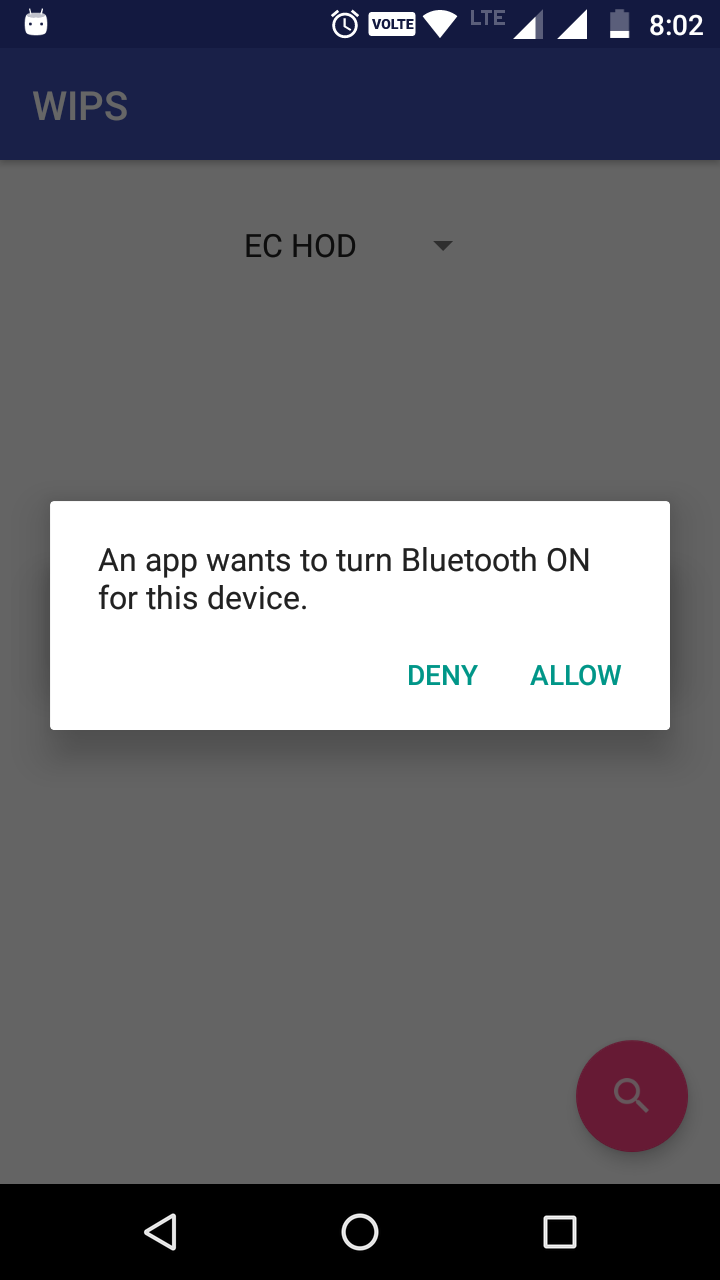
\includegraphics[width=.25\textwidth]{bl.png}    
		\caption{Asks to turn on Bluetooth}.
		\label{fig5}
	\end{center}
\end{figure}
\begin{figure}[!h]
	\begin{center}
		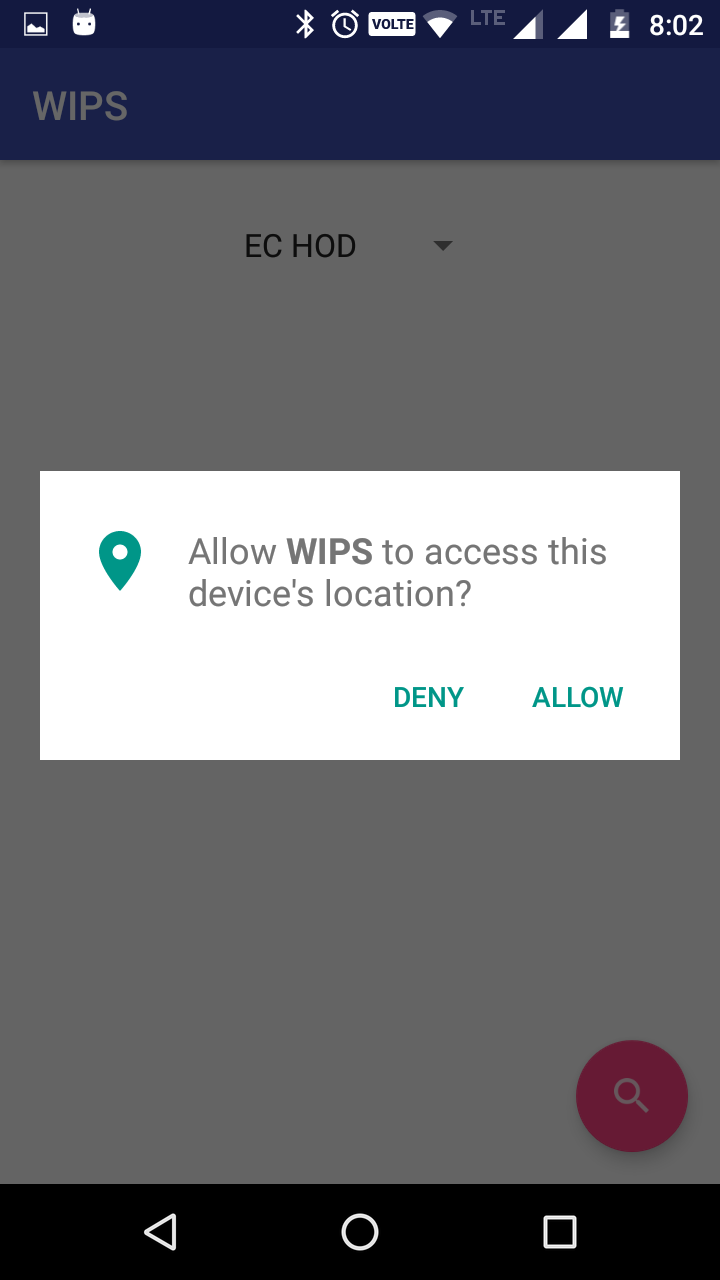
\includegraphics[width=.25\textwidth]{loc.png}    
		\caption{Asks LOCATION permission}.
		\label{fig6}
	\end{center}
\end{figure}
\begin{figure}[!h]
	\begin{center}
		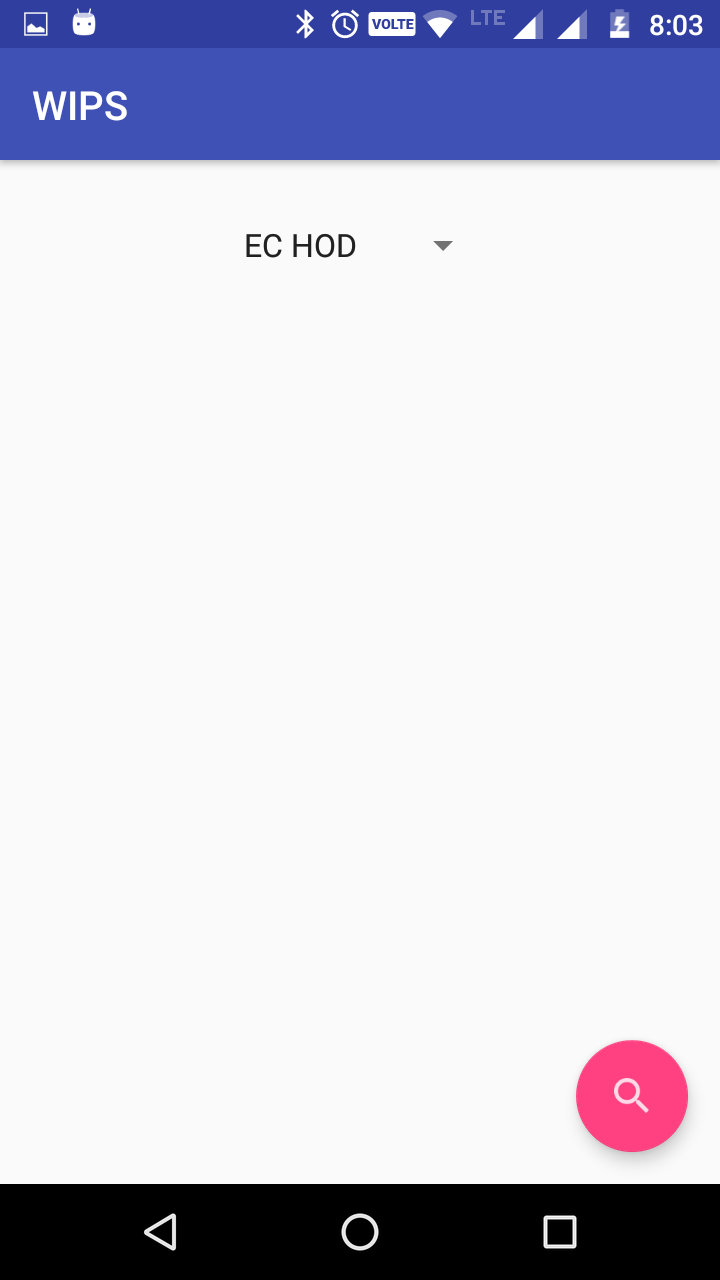
\includegraphics[width=.25\textwidth]{app.png}    
		\caption{Asks Destination}.
		\label{fig7}
	\end{center}
\end{figure}
\begin{figure}[!h]
	\begin{center}
		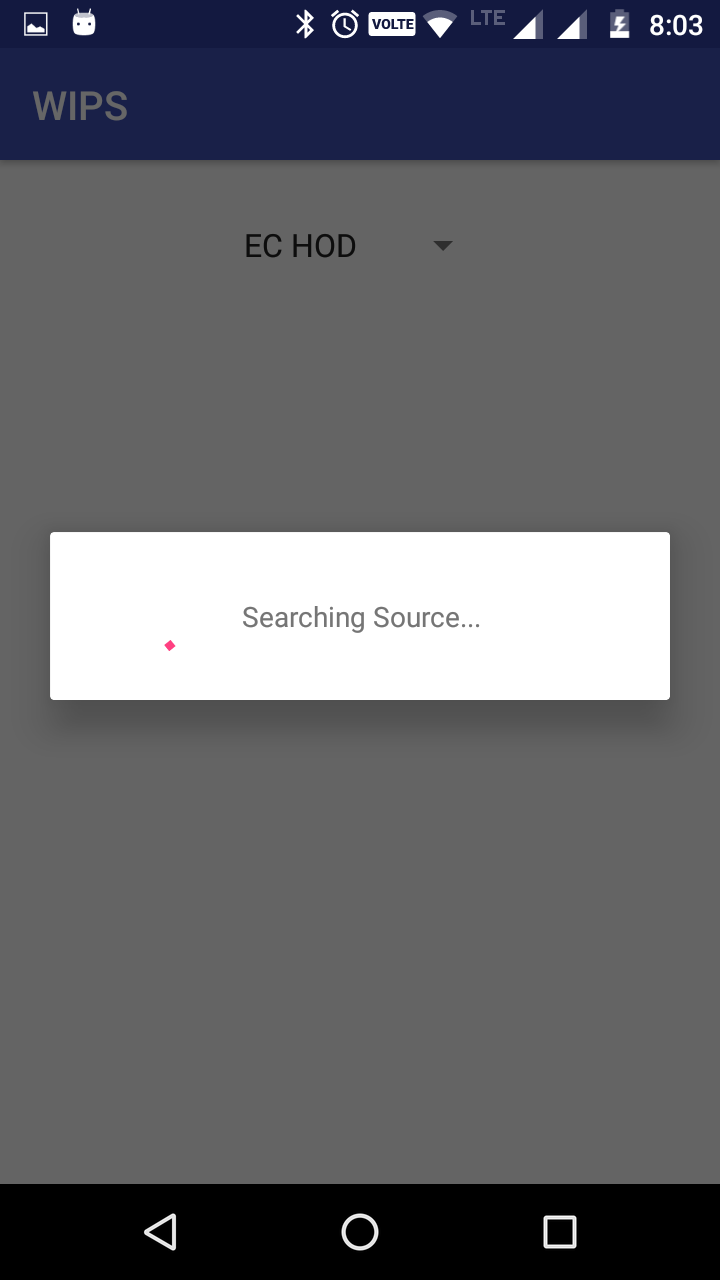
\includegraphics[width=.25\textwidth]{app1.png}    
		\caption{Searches Source}.
		\label{fig8}
	\end{center}
\end{figure}
\begin{figure}[!h]
	\begin{center}
		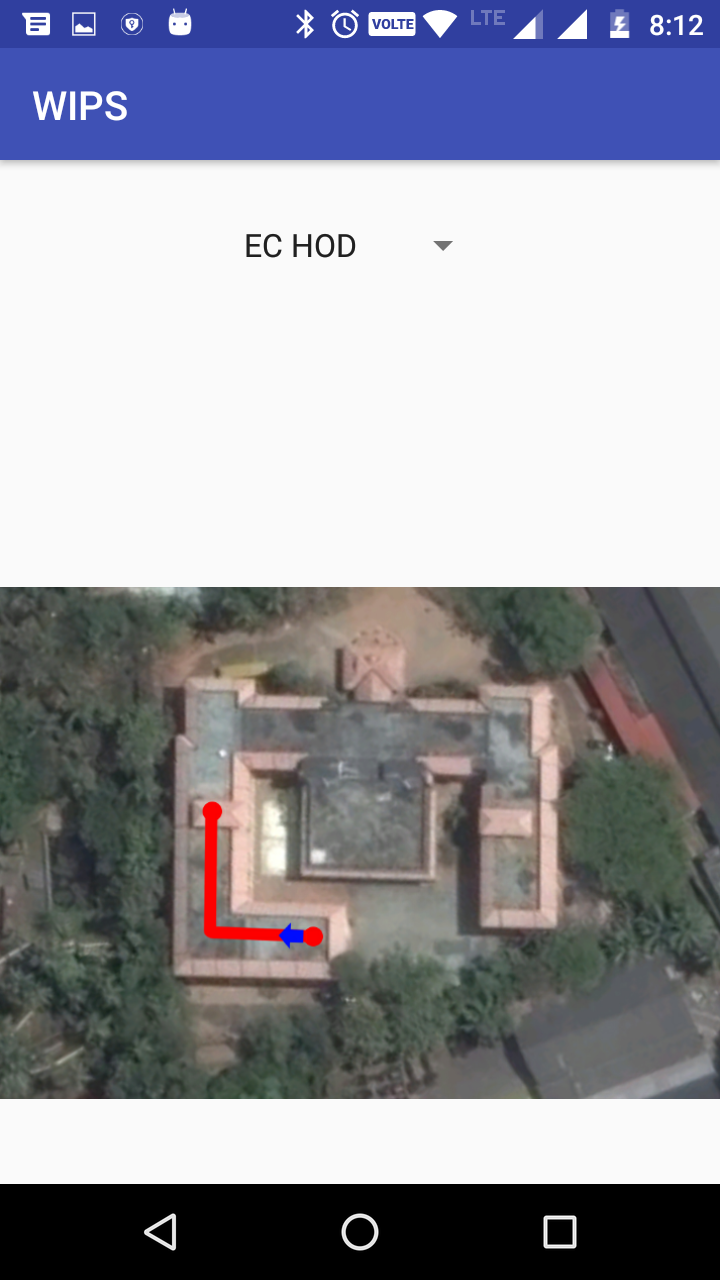
\includegraphics[width=.25\textwidth]{app2.png}    
		\caption{Path}.
		\label{fig9}
	\end{center}
\end{figure}
\begin{figure}[!h]
	\begin{center}
		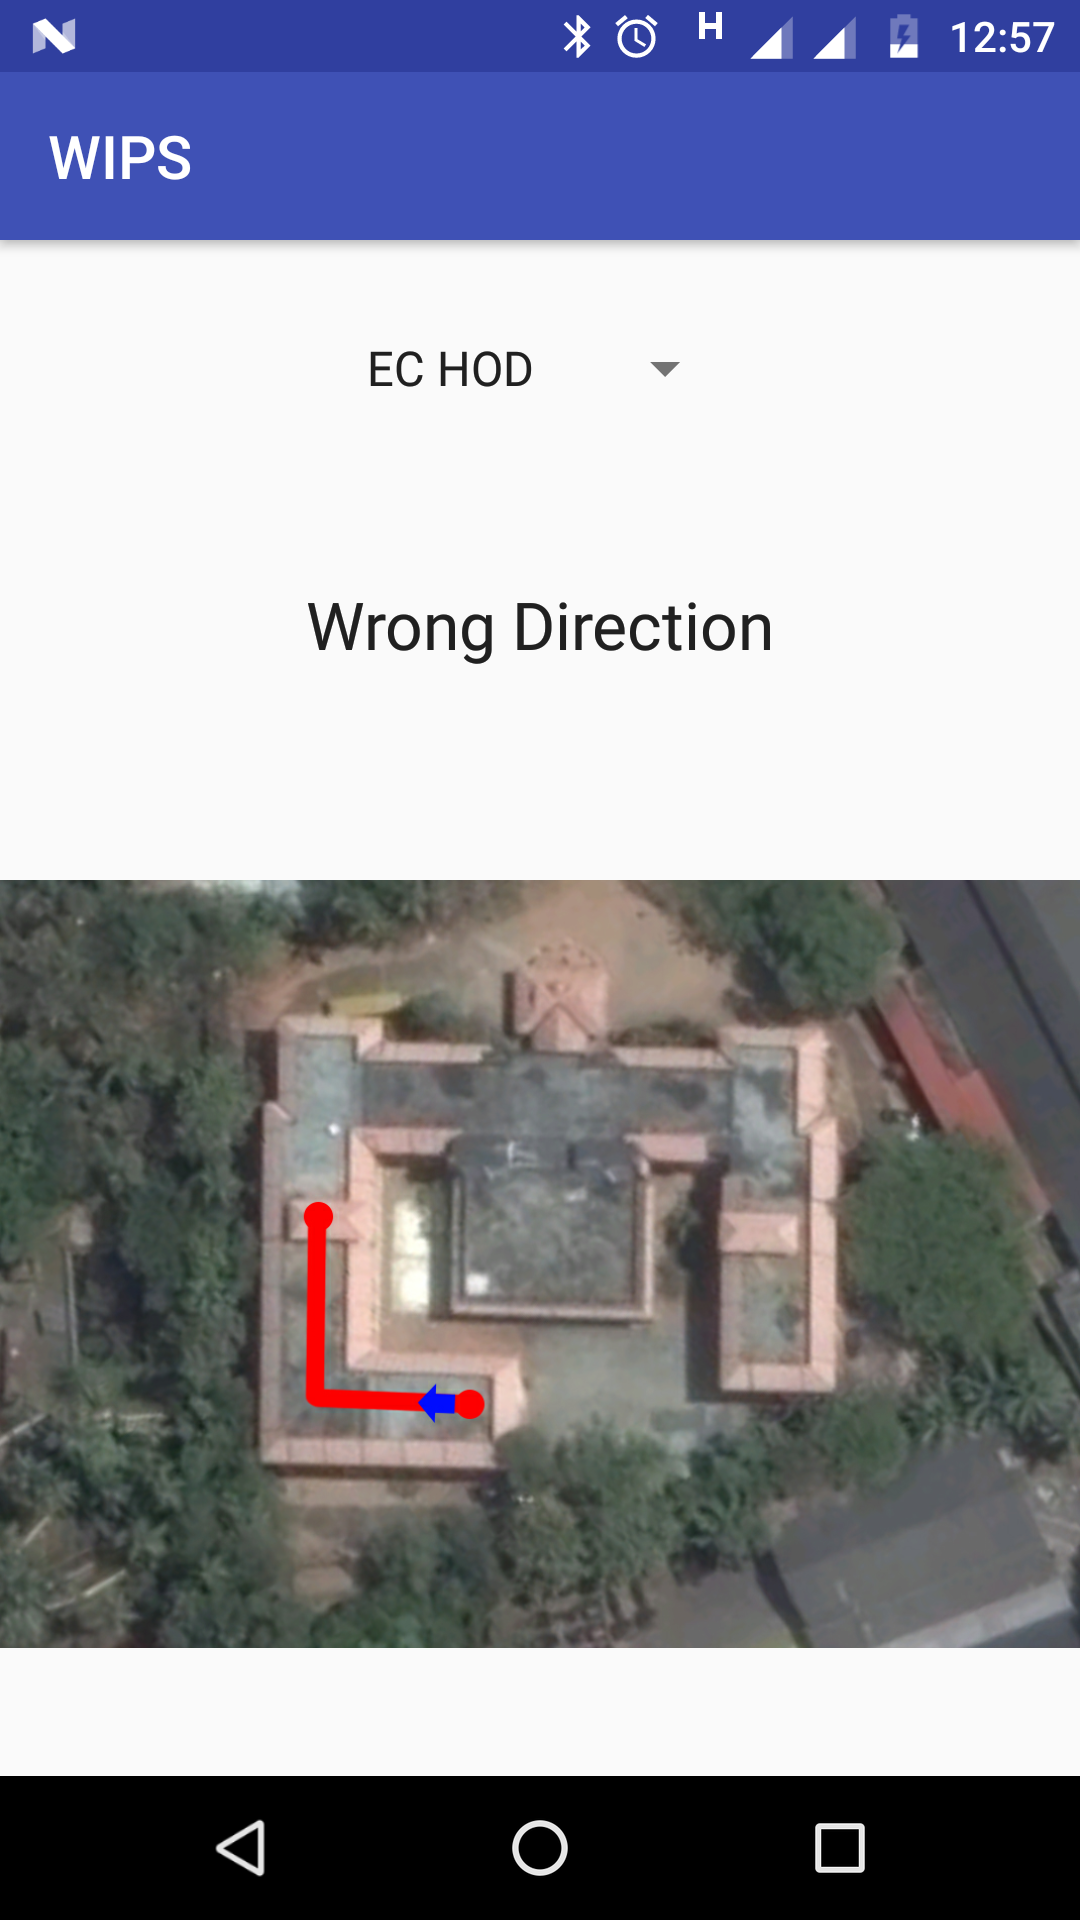
\includegraphics[width=.25\textwidth]{app5.png}    
		\caption{Notifies Wrong Direction}.
		\label{fig12}
	\end{center}
\end{figure}
\begin{figure}[!h]
	\begin{center}
		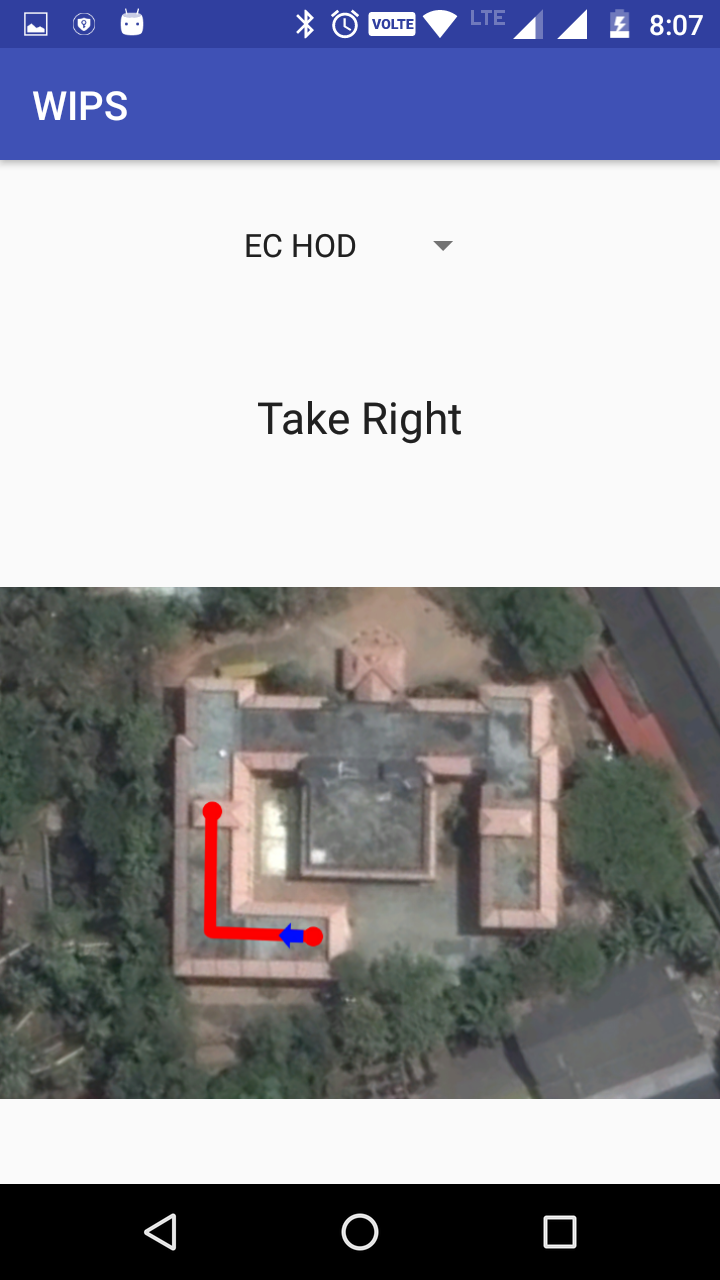
\includegraphics[width=.25\textwidth]{app3.png}    
		\caption{Notifies to turn right}
		\label{fig10}
	\end{center}
\end{figure}
\begin{figure}[!h]
	\begin{center}
		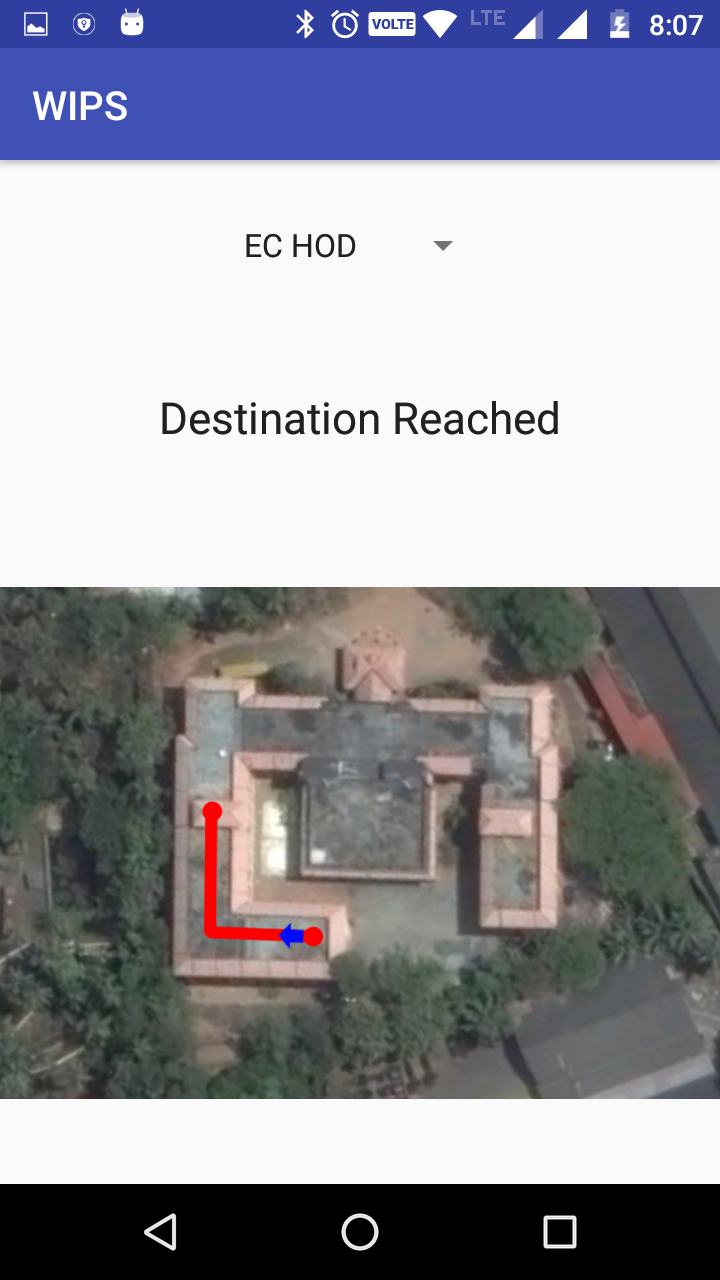
\includegraphics[width=.25\textwidth]{app4.png}    
		\caption{Notifies that desired destination has reached}
		\label{fig11}
	\end{center}
\end{figure}
\renewcommand\chaptername{CHAPTER}
\chapter{CONCLUSION AND FUTURE WORK}
\paragraph{} The main objective of the system is to navigate a user from his/her current position to the specified destination. Beacons are used for the system. Beacons use BLE technology. BLE technology is used since GPS and WiFi technologies are not efficient for the system. The main advantage of the system is that it consumes low power as it uses BLE technology. The system is an advantage for handicaps and an added luxury for others.
\paragraph{} The applications are :
\begin{itemize}
	\item Malls
	\item Hospital
	\item Multi storey building
\end{itemize}
\section{The advantages of using beacons in retail environments}
\paragraph{}Beacons offer several advantages to retailers looking to capture the attention of customers. They generate engagement between the customer and the business, and offer rewards to customers that choose to interact.  This builds customer loyalty and trust, while also providing retailers opportunities for strategic personalization.
\paragraph{}For example, if beacon technology can provide a retailer with the age, gender, and spending habits of a consumer, they can instantly utilize that information to send them push notifications for a promotion or product that they feel the consumer is likely to want. Beacons allow retailers to instantaneously adapt their marketing efforts to individual consumers, a strategy that can prove much more effective than trying to appeal to a broad target demographic.
\section{Potential drawbacks to implementing beacon technology}
\paragraph{}This great resource has not been without its setbacks. Retailers have found that consumers tend to get easily annoyed by receiving too many push notifications, and will stop using apps if they receive more than one in a short amount of time. In addition, not everyone has Bluetooth technology enabled on their phone.
\section{The unanticipated advantages of using beacons in retail environments}
\paragraph{}Despite the relatively slow growth of beacon technology and unforeseen obstacles, it has proven to be incredibly useful for something very powerful: data collection. When integrated with a business’s CRM system, beacons can track everything from footfalls, purchases through apps, loyalty and marketing effectiveness, service quality, queue abandonment, returning visitors, and a wide variety of metrics that can help businesses improve their marketing efforts and optimize the customer experience.
\paragraph{}Though the future of beacons may look different than originally anticipated, there is no denying that they will continue to adapt to provide valuable information and services to retail businesses, allowing them drive sales through targeted marketing efforts and gain greater insight into their customer base.
\section{The Future of Evolving Beacon Technology}
\paragraph{}This amazing technological advancement is set to revitalize retail and other business in multiple ways while offering a variety of benefits for companies and consumers. As businesses continue to create new technology integration strategies, beacons' uses will likely continue to grow. Examples of some current benefits include:
\begin{itemize}
	\item Create personalized messages to greet customers: When beacons are placed at the entrance and/or exit to a business, this offers an excellent opportunity to send personalized welcome or farewell messages to enhance the customer experience and automate exit surveys
	\item Guide people to specific areas or products: Beacons can direct people where they need to go — whether that's the restroom, customer service department or shelves that contain specific products
	\item Take in-store experiences to a new level: From sending coupon offers while customers shop to expanding a business's ability to distribute helpful advertisements and promotions — such as games, product models and surveys — beacons elevate consumer experiences by making it easier for customers to interact with their favorite brands.
\end{itemize}
\paragraph{}Since iBeacons were first introduced in 2013, these tools have propelled the evolution of technology. From business information technology to retail, the growing interconnectivity that beacons represent offers new, exciting opportunities for consumers and businesses alike.
\paragraph{}Considering the benefits that beacons already bring to the table, the future of beacon technology should be nothing short of fascinating. In this fast-paced digital world, where evolving technology progresses at a rapid rate, keeping your skills sharp is one of the most important keys to remaining competitive in the job market.

\newpage
\addcontentsline{toc}{chapter}{REFERENCES}
\renewcommand\bibname{\textbf{REFERENCES}}
\bibliographystyle{ieeetr}

\begin{thebibliography}{1}
	
	\bibitem{Android}
	Android, Wikipedia, https://en.wikipedia.org/wiki/Android\_(operating\_system)
	
	\bibitem{AndroidStudio}
	Android Developer, https://developer.android.com/studio/index.html
	
	\bibitem{Beacon}
	Beacon, Wikipedia, https://en.wikipedia.org/wiki/Beacon.
	
	\bibitem{IBeacon}
	iBeacon, Wikipedia, https://en.wikipedia.org/wiki/IBeacon.
	
\end{thebibliography}
\end{document}
